We first convert audio files into spectrogram images, and for each segments we use Hanning windows with \%75 overlap. Notice the case that in a processed grayscale image most area was occupied by the random noise. What we want is to get rid of the background noise completely and increase the contrast between real signal and the background. Given the several different algorithm tested, the median clipping algorithm works best because it not only removes most background noise, but also capture the sound feature clearly and precisely.

\begin{center}
\begin{tabular}{cc}
\begin{minipage}{1.8truein}
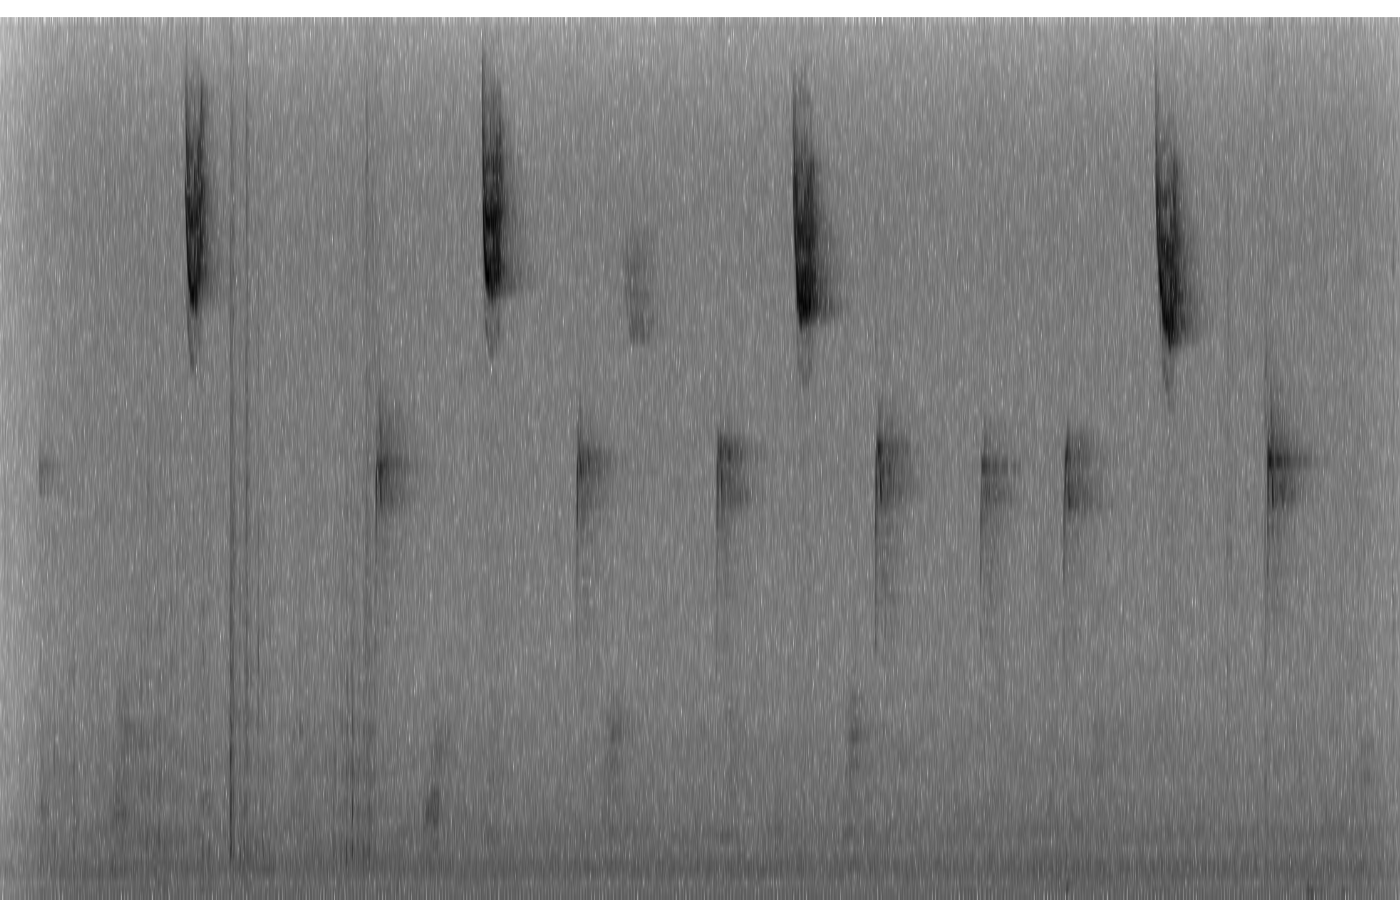
\includegraphics[height=1truein]{images/original}
\end{minipage}&
\begin{minipage}{1.8truein}
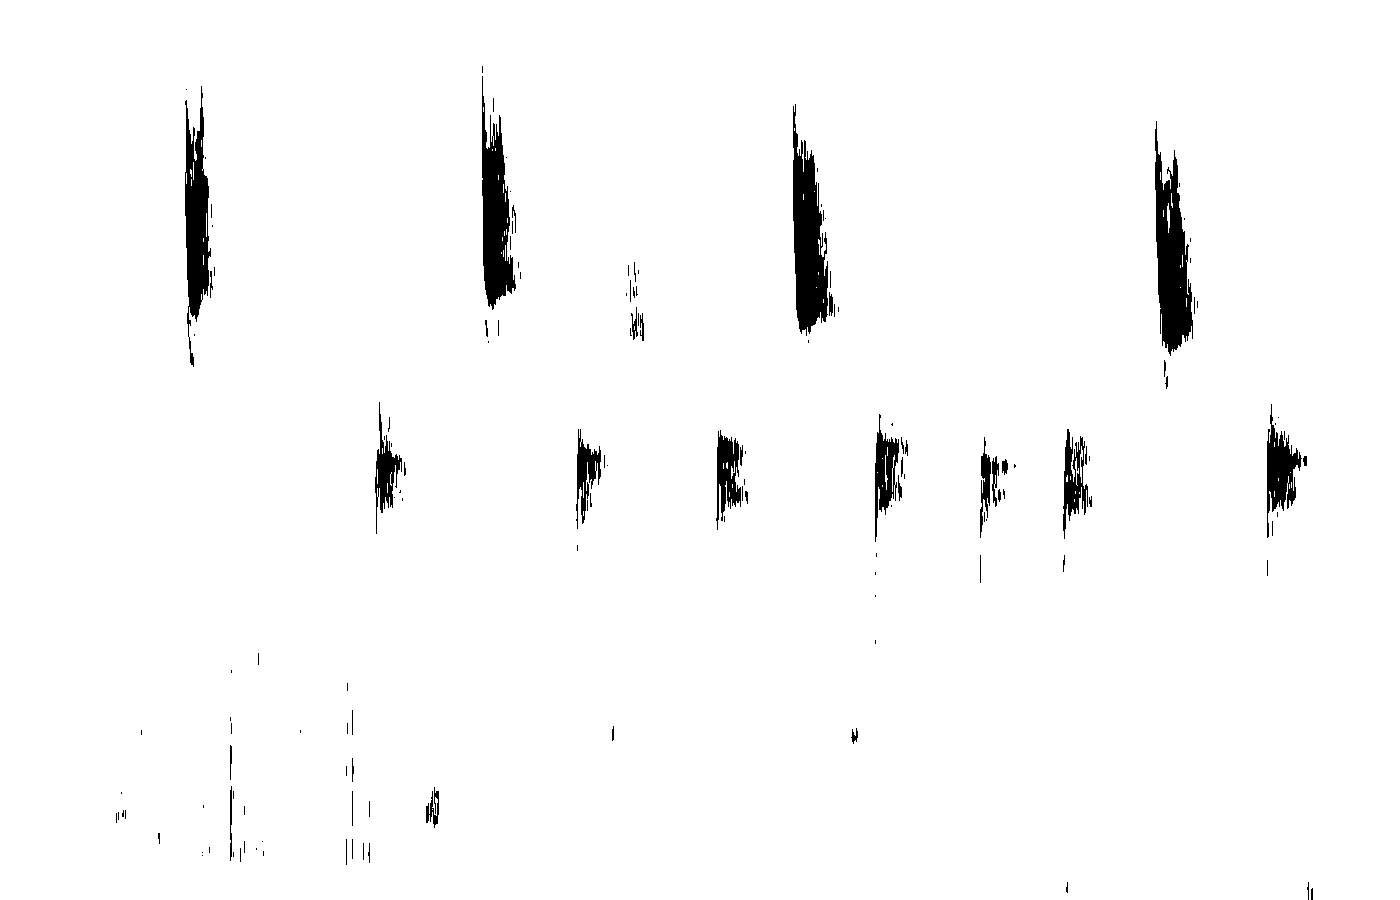
\includegraphics[height=1truein]{images/Median_clipped}
\end{minipage}\\
\begin{minipage}{1.8truein}
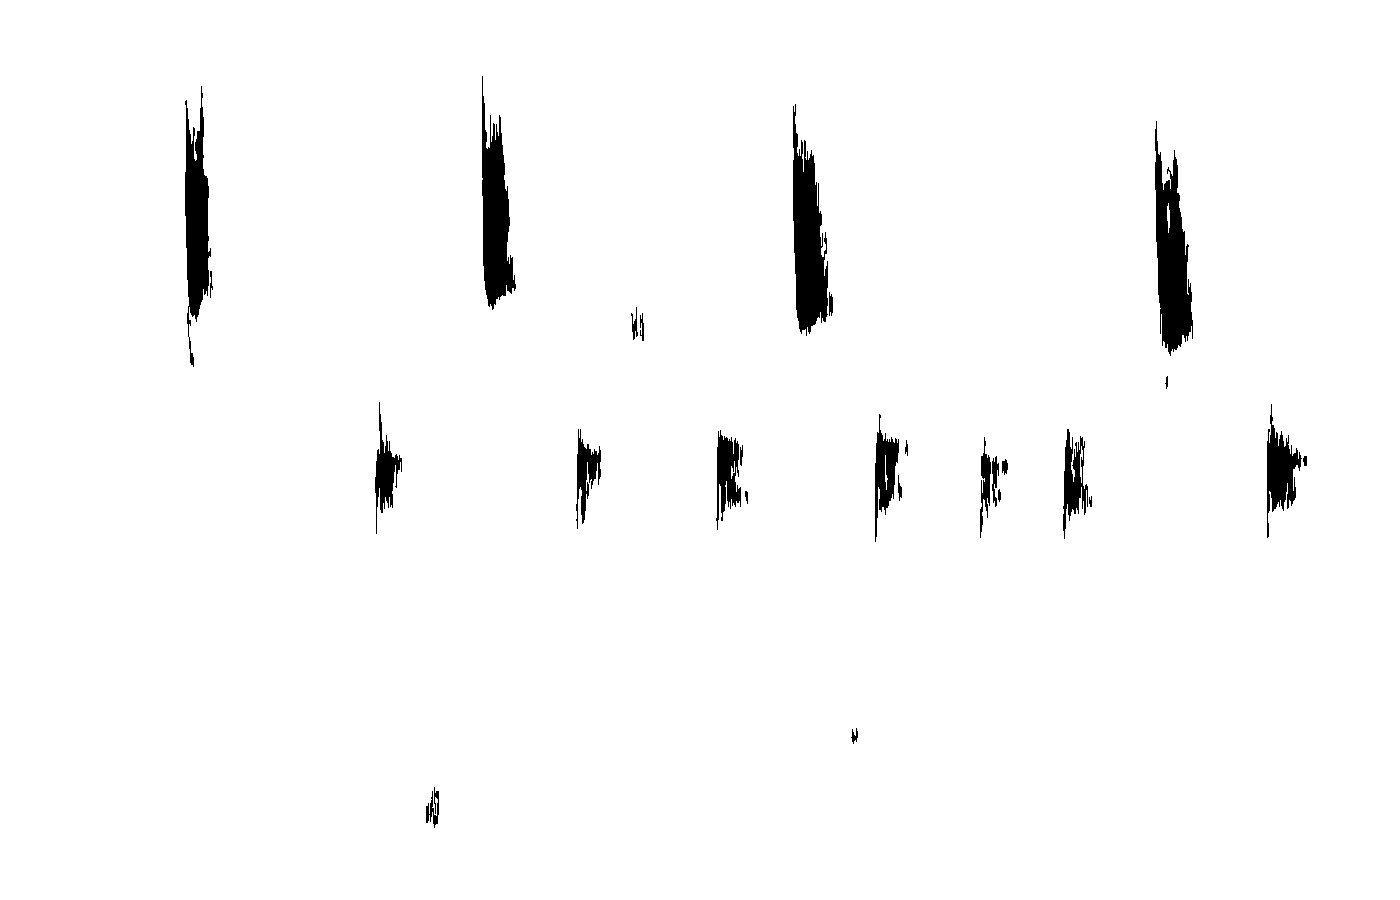
\includegraphics[height=1truein]{images/Eroded_and_propagated}
\end{minipage}&
\begin{minipage}{1.8truein}
\includegraphics[height=1truein]{images/labeled}
\end{minipage}\\
\end{tabular}
\end{center}
